\section{Case Study Details}
An ideal practice of Modelgo is to assess real-world ML projects and detect their potential license compliance issues. 
However, this can be challenging in practice due to three present situations:

(1) Prevalent Licensing Disorganization in ML Projects: Many ML projects lack organized licensing information, making it difficult to ascertain the licenses of individual components.

(2) Lack of Development Lifecycle Information for ML Reusing: ML reusing often occurs without a clear record, making it hard to trace the origins and licenses of components used.

(3) Non-compliance within Datasets: Crowdsourced datasets often suffer from license non-compliance issues~\cite{rajbahadur2021can}, making the licenses (usually permissive) declared by dataset collectors invalid.

Consequently, directly analyzing real-world ML projects may result in uncertainty, over-optimistic results, and often fail to detect any license conflicts.
Therefore, to validate Modelgo, we have designed five ML scenarios rendered using 15 common data sources and 11 models that cover 5 modalities and 7 tasks, respectively.
Table~\ref{tab:works} shows the specifications of the involved data sources and models, whose licenses include copyleft, permissive, public domain, and no public license~\footnote{Some data sources contain crowdsourced content with multiple licenses, and we selected a non-public domain license among them.}.
Furthermore, our case studies can cover all events listed in Table~\ref{tab:analysis}, and the their details and findings are provided in the following section.

It's worth noting that, as a license compliance analysis tool, Modelgo's goal is to report potential legal risks in ML projects related to licenses.
It is not designed to address legal interpretation issues such as copyrightability of the final work, assessing copyright infringement, or establishing authorship, which typically require verification by a court of law in different regions~\cite{national1979final, hedrick2019ithink, margoni2018artificial}.


\begin{table}[t]
    \caption{Specifications of AI components used in case studies, which include \textcolor{Copyleft}{Copyleft License}, \textcolor{Permissive}{Permissive License}, \textcolor{Public}{Public Domain Licens} and No Public License.}
    \footnotesize
    \label{tab:works}
    \begin{tabular}{|p{1.6cm}|p{3cm}|p{0.6cm}|p{1.7cm}|}
        \hline
        \rowcolor[gray]{.8}
        \textbf{Work Name} & \textbf{License Name} & \textbf{Type} & \textbf{Modality/Usage}  \\ \hline
        Wikipedia & \textcolor{Copyleft}{CC-BY-SA-4.0} & \multirow{15}{*}{Data} & \multirow{6}{*}{Text}   \\ \cline{1-2}
        StackExchange & \textcolor{Copyleft}{CC-BY-SA-4.0}  &  &    \\ \cline{1-2}
        FreeLaw & CC-BY-ND-4.0 &  &   \\ \cline{1-2}
        arXiv & \textcolor{Copyleft}{CC-BY-NC-SA-4.0} &  &   \\ \cline{1-2}
        PubMed & \textcolor{Copyleft}{CC-BY-NC-SA-4.0} &  &    \\ \cline{1-2}
        Deep-sequoia & CC-BY-NC-ND-4.0 &  &   \\ \cline{1-2} \cline{4-4}

        Midjourney Gen & CC-BY-NC-ND-4.0 &  & \multirow{6}{*}{Image}  \\ \cline{1-2}
        Flickr & \textcolor{Copyleft}{CC-BY-NC-SA-4.0} &  &   \\ \cline{1-2}
        StockSnap & \textcolor{Public}{CC0-1.0} &  &   \\ \cline{1-2}
        Wikimedia & \textcolor{Copyleft}{CC-BY-SA-4.0} &  &   \\ \cline{1-2}
        OpenClipart & \textcolor{Public}{CC0-1.0} &  &   \\ \cline{1-2} \cline{4-4}
        
        ccMixter & \textcolor{Permissive}{CC-BY-NC-4.0} & & \multirow{2}{*}{Voice}  \\ \cline{1-2}
        Jamendo & CC-BY-NC-ND-4.0 &  &   \\ \cline{1-2} \cline{4-4}
        
        Thingverse & \textcolor{Copyleft}{CC-BY-NC-SA-4.0} &  & 3D model  \\ \cline{1-2} \cline{4-4}

        Vimeo & CC-BY-NC-ND-4.0 &  & Video  \\ \hline

        Baize & \textcolor{Copyleft}{GPL-3.0} & \multirow{11}{*}{Model} & \multirow{4}{*}{Text Generation}   \\ \cline{1-2}
        BLOOM & \textcolor{Permissive}{BigScience-BLOOM-RAIL-1.0} & &   \\ \cline{1-2}
        Llama2 & \textcolor{Permissive}{Llama2} & &   \\ \cline{1-2}
        BigTranslate & \textcolor{Copyleft}{GPL-3.0} & &   \\ \cline{1-2} \cline{4-4}

        BERT & \textcolor{Permissive}{Apache-2.0} &  & Fill-Mask   \\ \cline{1-2} \cline{4-4}

        Stable Diffusion & \textcolor{Permissive}{CreativeML-OpenRAIL-M} & & Text to Image  \\ \cline{1-2} \cline{4-4}

        MaskFormer & \textcolor{Permissive}{CC-BY-NC-4.0} & & Image  \\ \cline{1-2}
        DETR & \textcolor{Permissive}{Apache-2.0} & & Segmentation \\ \cline{1-2} \cline{4-4}

        Whisper & \textcolor{Permissive}{MIT} & & Voice to Text  \\ \cline{1-2} \cline{4-4}

        X-Clip & \textcolor{Permissive}{MIT} & & Video to Text  \\ \cline{1-2} \cline{4-4}

        I2VGen-XL & CC-BY-NC-ND-4.0 & & Image to Video  \\ \hline

        \end{tabular}
\end{table}

\subsection{CASE \Romannum{1} : Corpus Combination}

\begin{figure}[h]
    \centering
    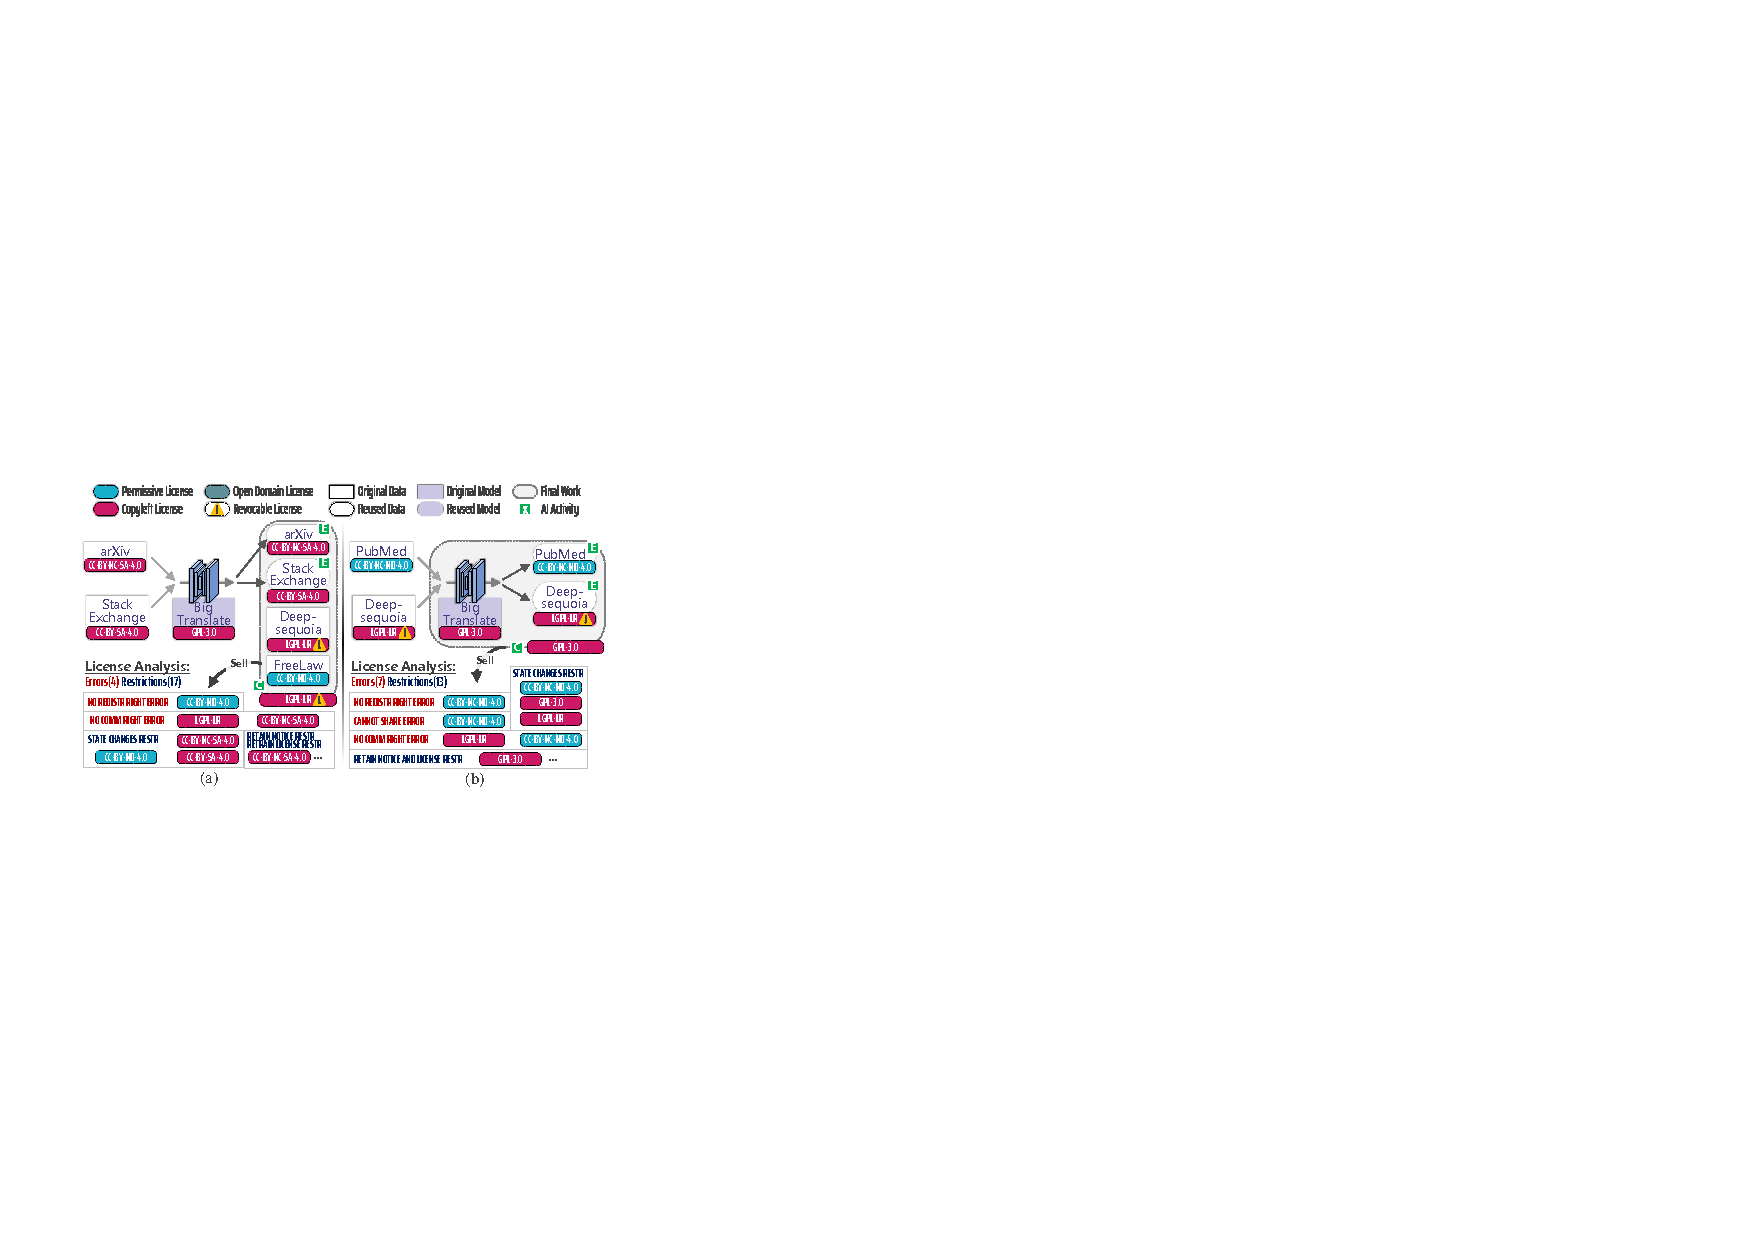
\includegraphics[width=\linewidth]{fig/case1.pdf}
    \caption{CASE \Romannum{1}: Corpus Combination. (a) Example of copyleft proliferation rules ; (b) Example of LGPL-LR exemption and no public license. AI Activities: \boxed{\text{E}}mbed, \boxed{\text{C}}ombine.}
    \Description{}
    \label{fig:case1}
\end{figure}

Our first case is corpus combination, which is very common in crowdsourced LLM datasets~\cite{gao2020the, penedo2023refinedweb, kocetkov2023stack}. 
Additionally, we also consider scenarios where the corpus is extended with the help of translation LLM.
As shown in Figure~\ref{fig:case1} (a), we first translate\footnote{In our cases, we treat translation as a specific form of embedding with a natural language output.} \textit{arXiv} and \textit{Stack Exchange} using \textit{Big Translate} model, then we combine these translated corpuses with \textit{Deep-sequoia} and \textit{FreeLaw}.
This combined corpus is the final work, intended for commercial purposes.
Figure~\ref{fig:case1} (b) depicts a variation in which the final work is a combination of translated corpus and the LLM.
Note that, to simplify analysis, we treat these no public licenses, such as CC-BY-ND-4.0 and CC-BY-NC-ND-4.0, as permissive licenses with limitations on sharing derivatives, as they do not include any copyleft terms.
If not specified otherwise, the format of models and datasets is set to raw (i.e., modifiable), while the other supported formats are binary and SaaS.
%We have also consolidated some redundant results reported by intermediate reused components to simplify our figures.
The interpretation of license analysis results is as follows:

\boxed{\text{Results of CASE \Romannum{1} (a)}} 
The copyleft conditions about \textit{translation} of the CC licenses were triggered, which means that the translated corpuses are also covered by the original licenses.
As a result, the translated \textit{arXiv} and \textit{Stack Exchange} corpuses remain under the original copyleft CC ShareAlike licenses. 
However, combining these corpuses with another copyleft-licensed \textit{Deep-sequoia} corpus did not result in the multiple copyleft licenses error, as the combination with strong separate falls outside the proliferate coverage of LGPL-LR and CC ShareAlike licenses~\cite{creative2023artificial}.
But, the proliferation extended to the final work and force it to be licensed under LGPL-LR as well.
It is important to note that only the effort taken to combine the corpuses is under LGPL-LR, and the licensing action to the final work will not change the licenses of its components.

There are two types of errors according to Modelgo's assessment.
The first error arises from the CC-BY-NC-SA-4.0 license of the translated \textit{arXiv}, which doesn't grant the right of commercial use\footnote{This error also arises from \textit{arXiv} since it is a sub-work of the translated \textit{arXiv}, we will consolidate this type of redundant in the rest of the case studies.}. 
The second error is caused by the fact that the redistribution rights of FreeLaw are not granted to comply with CC-BY-ND-4.0.
There are also many restrictions, such as the final work must state the changes compared to the original work and must retain the licenses and notice files of the original works.
In addition, Modelgo also indicates that the granted rights of LGPL-LR are revocable, which poses a potential risk for further redistribution.

\boxed{\text{Results of CASE \Romannum{1} (b)}} 
Different from CASE \Romannum{1} (a), the final work in CASE \Romannum{1} (b) is licensed under another copyleft license GPL-3.0 from \textit{Big Translate}.
This is because LGPL-LR has a license proliferation exemption for reused results that are no longer classified as linguistic resources.
Consequently, the license of final work is proliferated by GPL-3.0.
Additionally, besides the rights not granted error arising from CC-BY-NC-ND-4.0, this no public license also explicitly prohibits any form of sharing derivatives, resulting in a cannot share error.

\boxed{Summary} 
% 结论:数据集的收集应该避免no public 和 不能商用的数据集,使用copyleft 的CC 数据集比较安全,但是其他GPL需要额外注意扩散范围

\subsection{CASE \Romannum{2} : Mixture of Experts}

\begin{figure}[h]
    \centering
    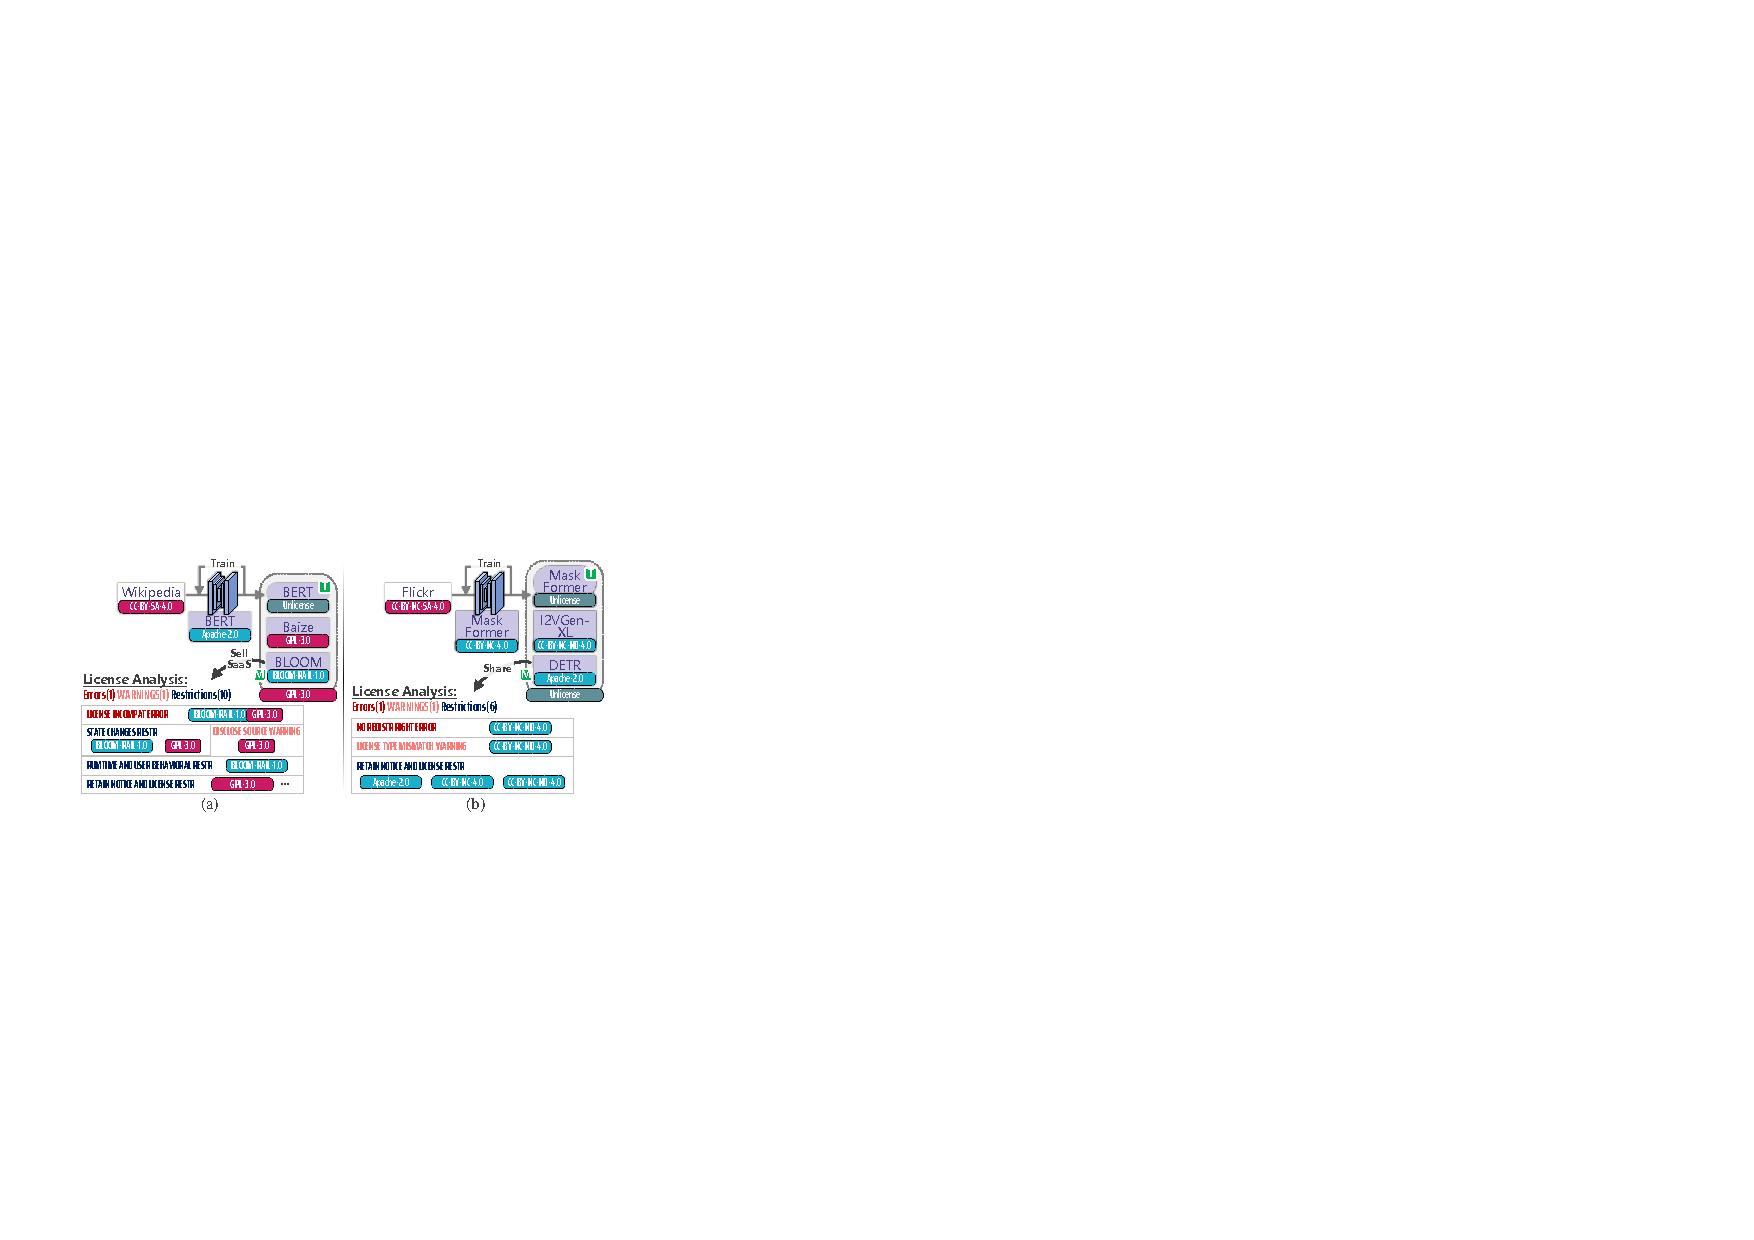
\includegraphics[width=\linewidth]{fig/case2.pdf}
    \caption{CASE \Romannum{2}: Mixture of Experts. (a) Source code disclosure of GPLed work; (b) Sharing work under CC NoDerivs. AI Activities: \boxed{\text{T}}rain, \boxed{\text{M}}oE.}
    \Description{}
    \label{fig:case2}
\end{figure}

In this case study, we consider the MoE scenario, in which we combine two models with a newly trained model using a gating network.
There are two variations in this case, each involving different models, training data, release policies (SaaS and sharing), as depicted in Figure~\ref{fig:case2} (a) and (b), respectively.
A real-wrold counterpart could be Wu Dao 2.0, which is a LLM trained using MoE technology with input from tens of thousands of experts~\cite{he2022fastermoe}.
Additionally, releasing models as a service is commonly observed in commercial AI applications such as chatGPT and Midjourney.

\boxed{\text{Results of CASE \Romannum{2} (a)}} 
There is still significant legal uncertainty regarding whether CC-licensed works can be applied to AI training~\cite{creative2023artificial}.
Since there is no explicit definition of AI training and corresponding restrictions for resulting models within the license text, we consider training as an undefined activity that falls outside the scope of CC agreements.
Therefore, even though the copyleft CC-BY-SA-4.0 license is used for \textit{Wikimedia}, the trained model \textit{BERT} does not trigger the license proliferation conditions and can be relicensed to Unlicense.
The final work's license is proliferated to GPL-3.0 from \textit{Baize}, as in CASE \Romannum{1} (b).

There is one warning in the assessment: the final work released as SaaS should remain open source or provide a readable copy of the source code to comply with GPL-3.0. 
Meanwhile, user behavioral restrictions also apply to the final work, as it is a derivative of \textit{BLOOM} governed by responsible AI conditions~\cite{contractor2022behavioral}.

\boxed{\text{Results of CASE \Romannum{2} (b)}} 
In this case study, we replaced experts with CV models. 
The assessment reveals that the final work cannot be shared, whether modified or not, even for non-commercial purposes, if the project includes CC NoDerivs licenses, as these licenses do not grant redistribution rights to the licensee.
This feature is helpful for licensors who intend to prohibit any derivation and commercialization of their models without the need to draft a custom proprietary license.
However, this disorganization of ML projects' licensing has a negative effect on the entire ecosystem.

\boxed{Summary} 

\subsection{CASE \Romannum{3} : Generation Pipeline}

\begin{figure}[h]
    \centering
    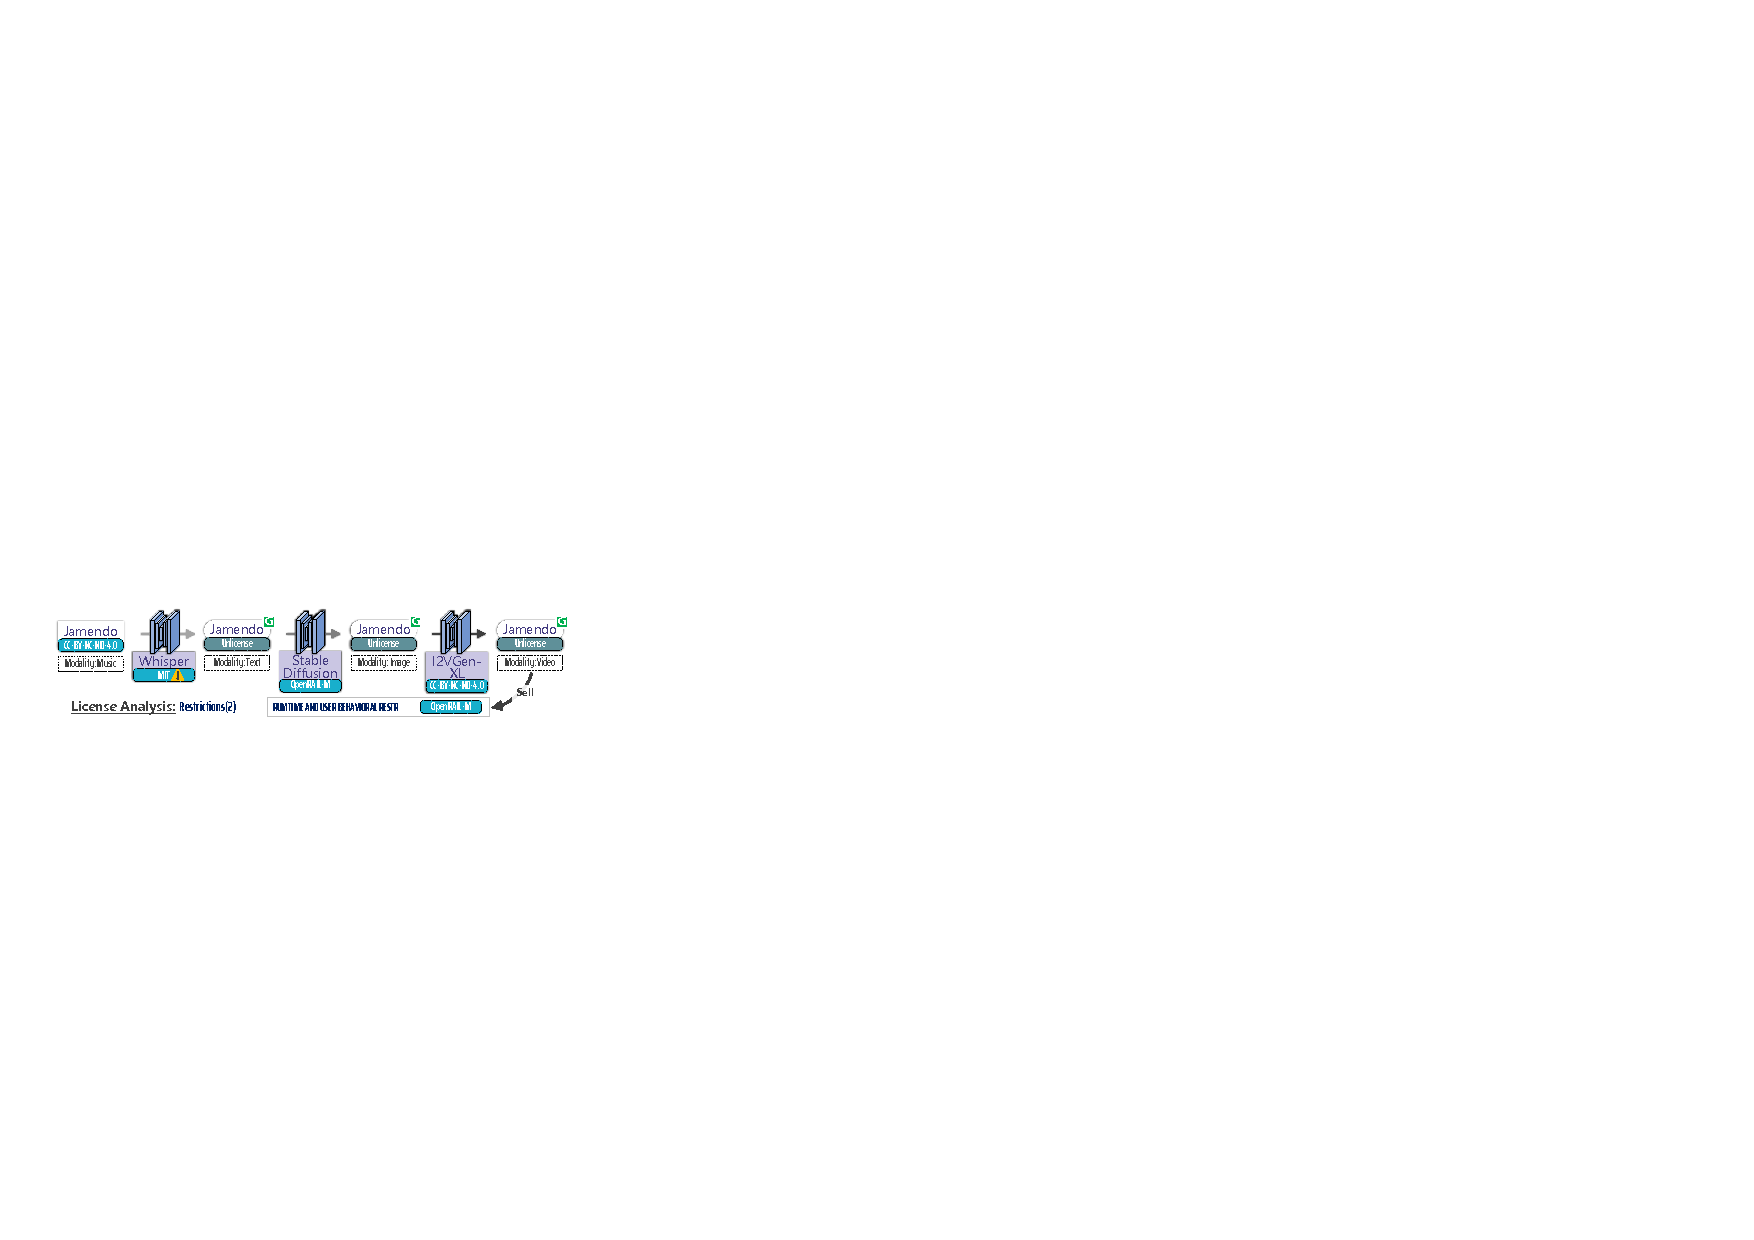
\includegraphics[width=\linewidth]{fig/case3.pdf}
    \caption{CASE \Romannum{3}: Generation Pipeline. AI Activities: \boxed{\text{G}}eneration}
    \Description{}
    \label{fig:case3}
\end{figure}

As shown in Table~\ref{tab:MLP}, artifact generation has become the most popular application of ML.
In this case study, we leverages generative models to produce data for different modalities in a pipeline fashion.
The final generated content is released for commercial use.

\boxed{\text{Results of CASE \Romannum{3}}} 
There is still an ambiguity in traditional OSS licenses and free content licenses when it comes to the use of licensed materials for generating artifacts.
From the perspective of the license agreement, this AI activity is permitted as long as the right to use is granted, and there are also no further claims for the generated content.
However, there is one restriction from OpenRAIL-M. 
The AI model license clearly defines the conditions for AI activities and applies copyleft-style restrictions to its licensed work. 
Therefore, once AI model licensed components are used in ML projects, all subsequent work should comply with these user behavioral restrictions, which can potentially lead to the final work becoming closed source~\cite{greenbaum2016the}.

\boxed{Summary} 
% Responsible AI 的 copyleft use behavioral 问题:历史累积 full spectrum

\subsection{CASE \Romannum{4} : Knowledge Transfer and Fusion}

\begin{figure}[h]
    \centering
    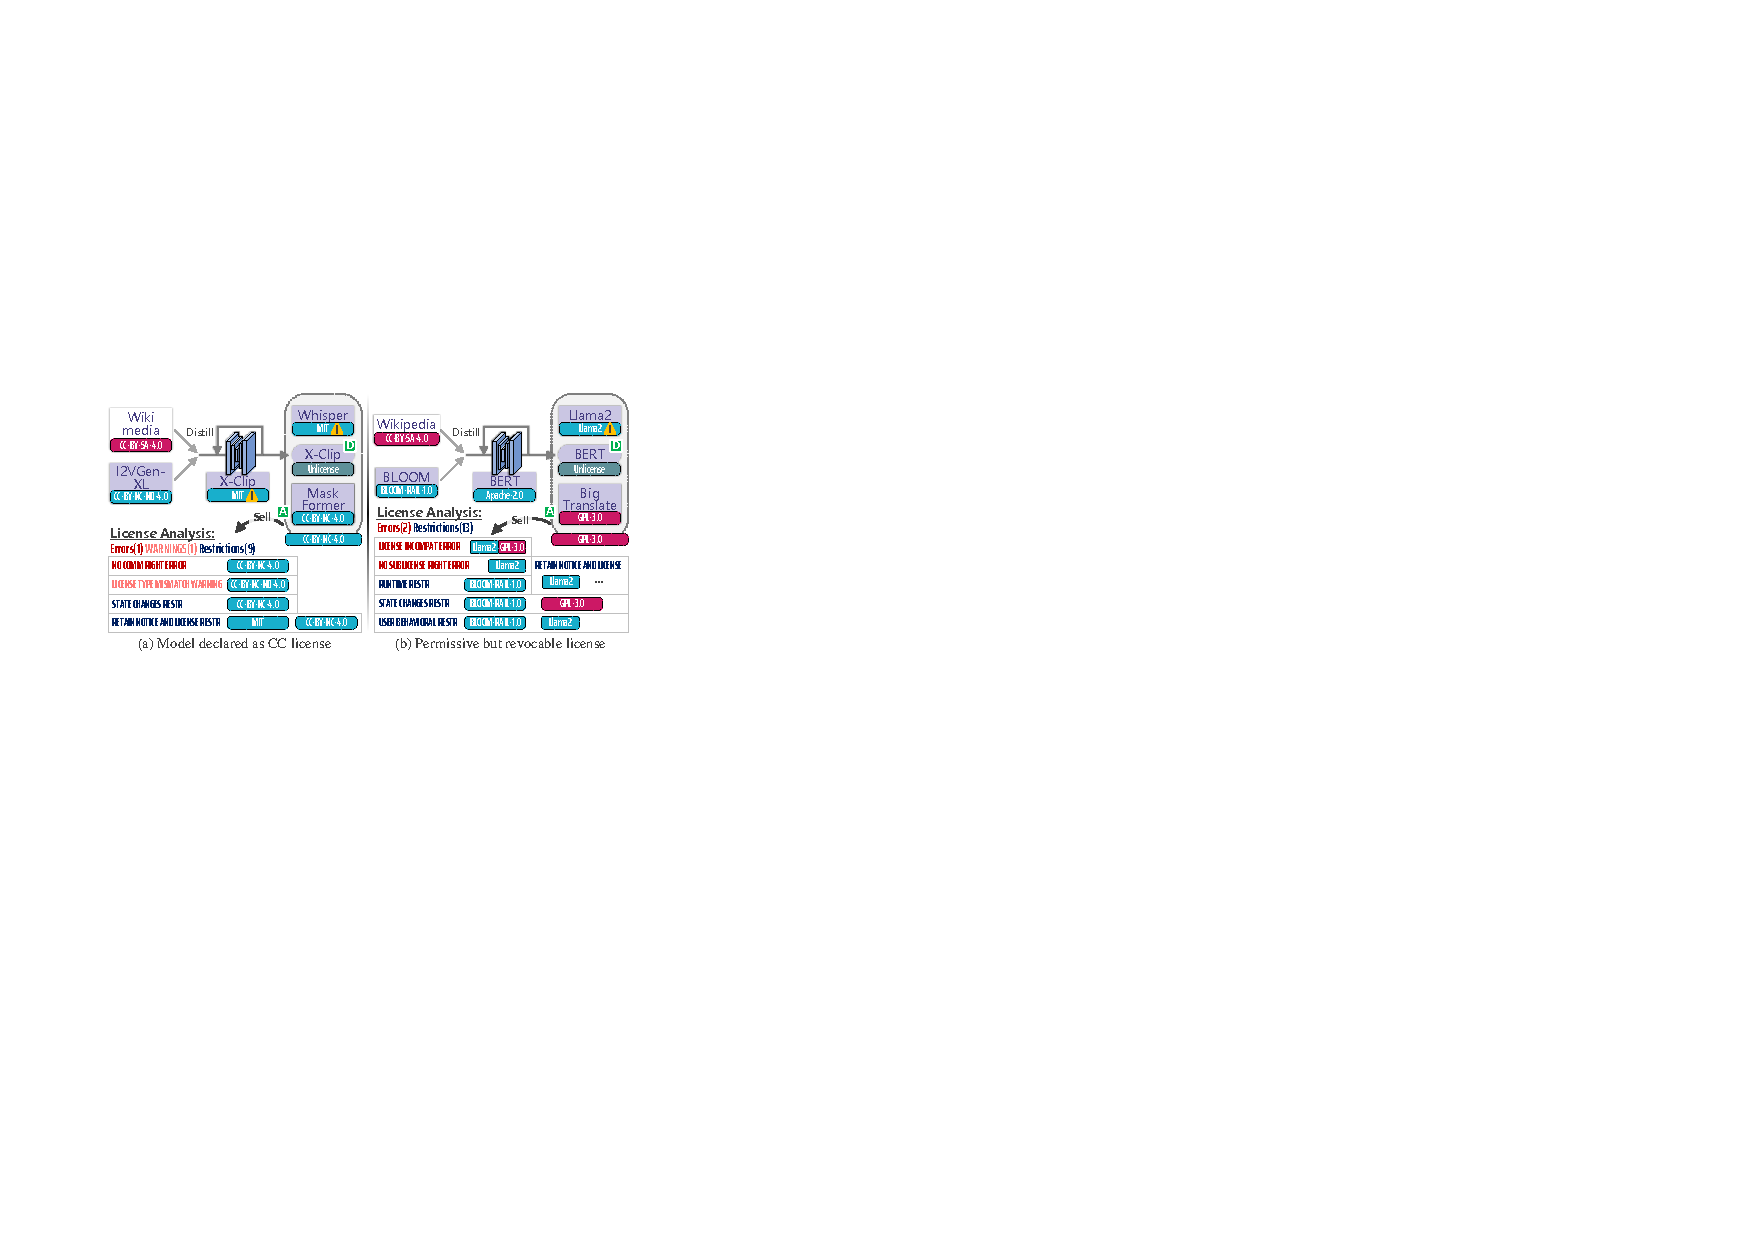
\includegraphics[width=\linewidth]{fig/case4.pdf}
    \caption{CASE \Romannum{4}: Knowledge Transfer and Fusion. AI Activities: \boxed{\text{D}}istillation, \boxed{\text{A}}malgamation.}
    \Description{}
    \label{fig:case4}
\end{figure}

The knowledge can be transferred or integrated from one model to another without the need for explicit code replication or linking. 
This is achieved through technologies such as Student-Teacher Learning~\cite{furlanello2018born}, Contrastive Learning~\cite{li2021model}, Federated Learning~\cite{mcmahan2017communication}, Model Fusion~\cite{lam2021model}, etc.
Traditional OSS license expose a loophole regarding these unique reusing methods from ML, and these methods also pose challenges for deep IP protection~\cite{peng2022intellectual}.
With the assistance of Modelgo, we further explore the compliance of these knowledge transfer methods within existing licensing framework.

\boxed{\text{Results of CASE \Romannum{4} (a)}} 
The distillation and amalgamation both yield a weak separation result from the original work, which can be interpreted as one form of modification.
Therefore, the final work should be under a CC-BY-NC-4.0, the same as \textit{Mask Former}.
However, the CC licenses do not define the terms for the materials used for distillation, so there is no effect from the copyleft licenses of \textit{Wikimedia} and \textit{I2VGen-XL}.
 
There is one error in the assessment. 
Since the modification of a CC NonCommercial licensed work cannot be relicensed according to its conditions, the amalgamated result face a no commercial rights error when commercialized.

\boxed{\text{Results of CASE \Romannum{4} (b)}} 

\boxed{Summary} 

\subsection{CASE \Romannum{5} : Remix Data}

\begin{figure}[h]
    \centering
    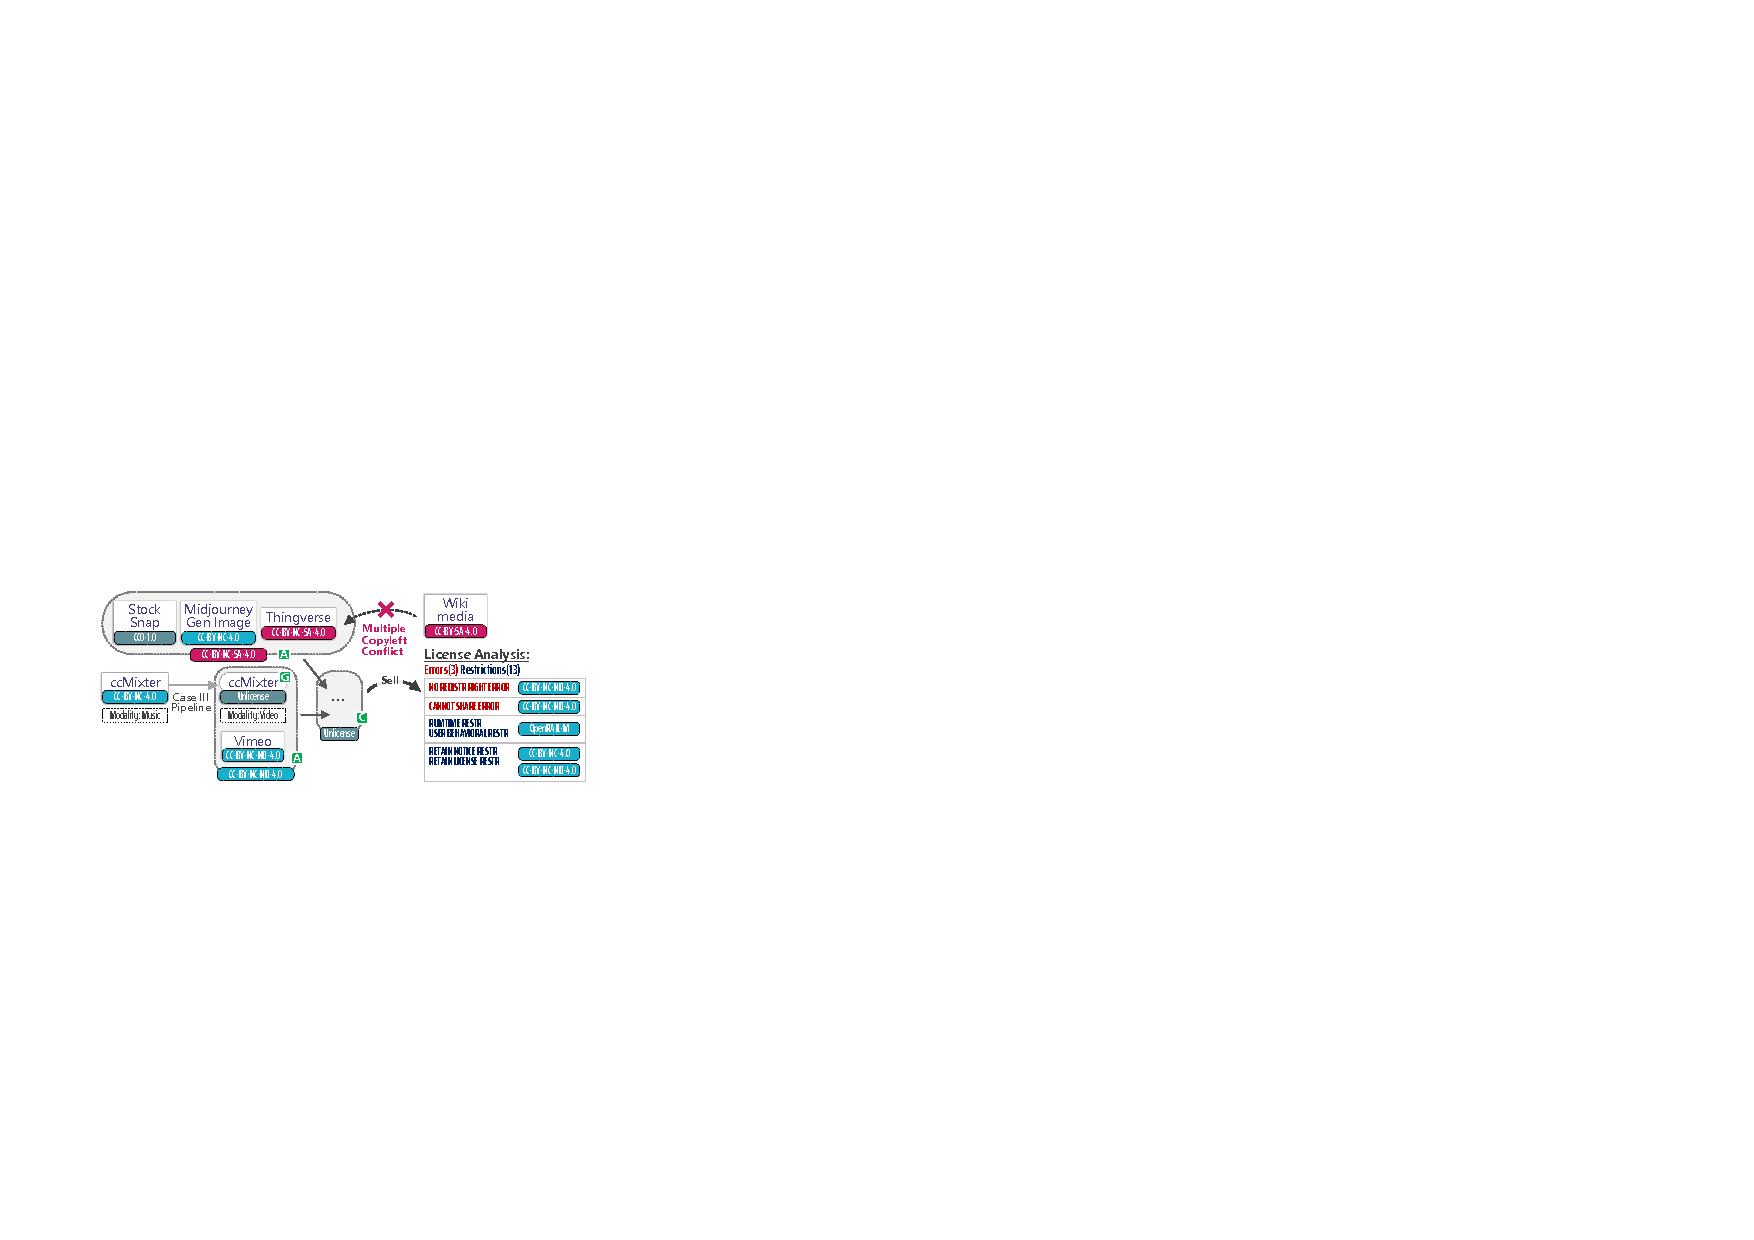
\includegraphics[width=\linewidth]{fig/case5.pdf}
    \caption{CASE \Romannum{5}: Remix Data.}
    \Description{}
    \label{fig:case5}
\end{figure}

\boxed{\text{Results of CASE \Romannum{5}}} 

\boxed{Summary} 